\ifx\allfiles\undefined
\documentclass[8pt a4paper, oneside, UTF8]{ctexbook}  % +  这一句是新增加的
\usepackage{amsmath}   % 数学公式
\usepackage[dvipsnames]{xcolor}
\usepackage{amsthm}    % 定理环境
\usepackage{amssymb}   % 更多公式符号
\usepackage{graphicx}  % 插图
\usepackage{mathrsfs}  % 数学字体
\usepackage{enumitem}  % 列表
\usepackage{geometry}  % 页面调整
\usepackage{unicode-math}
\usepackage{extarrows}
\usepackage{subfigure}
\usepackage{extarrows}
\usepackage{footnote}
\usepackage{svg}
\usepackage[colorlinks,linkcolor=black]{hyperref}
\usepackage{supertabular}
\usepackage{tcolorbox}
\usepackage{ulem}
\usepackage{framed}
\usepackage{float}
\usepackage{microtype}
\newcommand{\arccot}{\mathrm{arccot}\,}
\tcbuselibrary{breakable}
\tcbuselibrary{most}
\newcounter{problemname}
\newenvironment{solution}{\par\noindent\textbf{解答. }}{\par}
\newenvironment{note}{\par\noindent\textbf{题目\arabic{problemname}的注记. }}{\par}
\definecolor{shadecolor}{RGB}{241, 241, 255}
\newenvironment{problem}{\begin{shaded}\stepcounter{problemname}\par\noindent\textbf{题目\arabic{problemname}. }}{\end{shaded}\par}

\graphicspath{ {figure/},{../figure/}, {config/}, {../config/} }  % 配置图形文件检索目录
\linespread{1.2} % 行高

% 页码设置
\geometry{top=25.4mm,bottom=25.4mm,left=20mm,right=20mm,headheight=2.17cm,headsep=4mm,footskip=12mm}

% 设置列表环境的上下间距
\setenumerate[1]{itemsep=5pt,partopsep=0pt,parsep=\parskip,topsep=5pt}
\setitemize[1]{itemsep=5pt,partopsep=0pt,parsep=\parskip,topsep=5pt}
\setdescription{itemsep=5pt,partopsep=0pt,parsep=\parskip,topsep=5pt}

% 定理环境
% ########## 定理环境 start ####################################

% #### 将 config.tex 中的定理环境的对应部分替换为如下内容
% 定义单独编号,其他四个共用一个编号计数 这里只列举了五种,其他可类似定义(未定义的使用原来的也可)
\newtcbtheorem[auto counter, number within=section, list type=subsubsection, list inside=toc]{defn}{定义}
{
    colback=green!5,colframe=green!35!black,fonttitle=\bfseries, title={Comment \thetcbcounter}, list entry={Comment \thetcbcounter\quad}, %标题
    breakable, %支持跨页
    before upper={\parindent10pt\noindent},  % 支持缩进。\noindent:首行不缩进
    % left = 2mm, %文字离线框左边的边距
    % right = 1mm,%同上
    % top = 1mm,%同上
    % bottom = 1mm,%同上
    % arc is angular = 1mm, % 棱角线框
    % sharp corners, % 直角线框
    % enhanced,frame hidden, % 隐藏线框
    % enhanced, drop fuzzy shadow,  % 显示阴影
}
{def}

\newtcbtheorem[auto counter, number within=section, list type=subsubsection, list inside=toc]{lemma}{引理}
{
    colback=SeaGreen!10!CornflowerBlue!10,colframe=RoyalPurple!55!Aquamarine!100!,fonttitle=\bfseries, title={Comment \thetcbcounter}, list entry={Comment \thetcbcounter\quad}, %标题
    breakable, %支持跨页
    before upper={\parindent10pt\noindent},  % 支持缩进。\noindent:首行不缩进
    % left = 2mm, %文字离线框左边的边距
    % right = 1mm,%同上
    % top = 1mm,%同上
    % bottom = 1mm,%同上
    % arc is angular = 1mm, % 棱角线框
    % sharp corners, % 直角线框
    % enhanced,frame hidden, % 隐藏线框
    % enhanced, drop fuzzy shadow,  % 显示阴影
}
{lem}


\newtcbtheorem[auto counter, number within=section, list type=subsubsection, list inside=toc]{them}{定理}
{
    colback=Salmon!20, colframe=Salmon!90!Black,fonttitle=\bfseries, title={Comment \thetcbcounter}, list entry={Comment \thetcbcounter\quad}, %标题
    breakable, %支持跨页
    before upper={\parindent10pt\noindent},  % 支持缩进。\noindent:首行不缩进
    % left = 2mm, %文字离线框左边的边距
    % right = 1mm,%同上
    % top = 1mm,%同上
    % bottom = 1mm,%同上
    % arc is angular = 1mm, % 棱角线框
    % sharp corners, % 直角线框
    % enhanced,frame hidden, % 隐藏线框
    % enhanced, drop fuzzy shadow,  % 显示阴影
}
{them}
\newtcbtheorem[auto counter, number within=section, list type=subsubsection, list inside=toc]{criterion}{注}
{
    colback=CornflowerBlue!10,colframe=RoyalPurple!55!Aquamarine!100!,fonttitle=\bfseries, title={Comment \thetcbcounter}, list entry={Comment \thetcbcounter\quad}, %标题
    breakable, %支持跨页
    before upper={\parindent10pt\noindent},  % 支持缩进。\noindent:首行不缩进
    % left = 2mm, %文字离线框左边的边距
    % right = 1mm,%同上
    % top = 1mm,%同上
    % bottom = 1mm,%同上
    % arc is angular = 1mm, % 棱角线框
    % sharp corners, % 直角线框
    % enhanced,frame hidden, % 隐藏线框
    % enhanced, drop fuzzy shadow,  % 显示阴影
}
{cri}

\newtcbtheorem[auto counter, number within=section, list type=subsubsection, list inside=toc]{corollary}{推论}
{
    colback=Emerald!10,colframe=cyan!40!black,fonttitle=\bfseries, title={Comment \thetcbcounter}, list entry={Comment \thetcbcounter\quad}, %标题
    breakable, %支持跨页
    before upper={\parindent10pt\noindent},  % 支持缩进。\noindent:首行不缩进
    % left = 2mm, %文字离线框左边的边距
    % right = 1mm,%同上
    % top = 1mm,%同上
    % bottom = 1mm,%同上
    % arc is angular = 1mm, % 棱角线框
    % sharp corners, % 直角线框
    % enhanced,frame hidden, % 隐藏线框
    % enhanced, drop fuzzy shadow,  % 显示阴影
}
{cor}
% colback=red!5,colframe=red!75!black

% ######### 定理环境 end  #####################################

% ↓↓↓↓↓↓↓↓↓↓↓↓↓↓↓↓↓ 以下是自定义的命令  ↓↓↓↓↓↓↓↓↓↓↓↓↓↓↓↓

% 用于调整表格的高度  使用 \hline\xrowht{25pt}
\newcommand{\xrowht}[2][0]{\addstackgap[.5\dimexpr#2\relax]{\vphantom{#1}}}

% 表格环境内长内容换行  
\newcommand{\tabincell}[2]{\begin{tabular}{@{}#1@{}}#2\end{tabular}}

% 使用\linespread{1.5} 之后 cases 环境的行高也会改变,重新定义一个 ca 环境可以自动控制 cases 环境行高
\newenvironment{ca}[1][1]{\linespread{#1} \selectfont \begin{cases}}{\end{cases}}
% 和上面一样
\newenvironment{vx}[1][1]{\linespread{#1} \selectfont \begin{vmatrix}}{\end{vmatrix}}

\def\d{\textup{d}} % 直立体 d 用于微分符号 dx
\def\R{\mathbb{R}} % 实数域
\newcommand{\bs}[1]{\boldsymbol{#1}}    % 加粗,常用于向量
\newcommand{\ora}[1]{\overrightarrow{#1}} % 向量

% 数学 平行 符号
\newcommand{\pll}{\kern 0.5em/\kern -0.8em /\kern 0.5em}

% 用于空行\myspace{1} 表示空一行 填 2 表示空两行  
\newcommand{\myspace}[1]{\par\vspace{#1\baselineskip}}

\begin{document}
\begin{sloppypar}
    % \title{{\Huge{\textbf{高等数学笔记}}}}
\author{作者:于家崇}
\date{\today}
\maketitle                   % 在单独的标题页上生成一个标题

\thispagestyle{empty}        % 前言页面不使用页码
\begin{center}
	\Huge\textbf{前言}
\end{center}

If a job is worth doing,it's worth doing well
\begin{flushright}
	\begin{tabular}{c}
		\today \\ 如果一件事值得去做,那就值得去做好
	\end{tabular}
\end{flushright}

\newpage                      % 新的一页
\pagestyle{plain}             % 设置页眉和页脚的排版方式(plain:页眉是空的,页脚只包含一个居中的页码)
\setcounter{page}{1}          % 重新定义页码从第一页开始
\pagenumbering{Roman}         % 使用大写的罗马数字作为页码
\tableofcontents              % 生成目录

\newpage                      % 以下是正文
\pagestyle{plain}
\setcounter{page}{1}          % 使用阿拉伯数字作为页码
\pagenumbering{arabic}
% \setcounter{chapter}{-1}    % 设置 -1 可作为第零章绪论从第零章开始 
    \else
    \fi
    %  ############################ 正文部分
    \chapter{定积分(黎曼积分)}
    \section{定积分的概念}
    \begin{defn}{定积分的定义}{}
        若函数$f(x)$在区间$[a,b]$上有界,在$(a,b)$上任取$n-1$ 个分点$x_i(i=1,2,3,\cdots,n-1)$,定义$x_0=a$ 和$x_n=b$,且$a=x_0<x_1<x_2<x_3<\cdots<x_{n-1}<x_n=b$,记$\Delta x_k=x_k-x_{k-1},k=1,2,3,\cdots,n$.并任取一点$\xi_{k}\in[x_{k-1},x_{k}]$,记$\lambda=\max_{1\leq k \leq n}\{\Delta x_{k}\}$,若当$\lambda\to0$时,极限$\lim_{\lambda\to0}\sum_{k=1}^{n}f(\xi_{k})\Delta x_{k}$存在且与分点$x_i$及点$\xi_k$的取法无关,则称函数$f(x)$在区间$[a,b]$上可积,即
        $$
            \int_{a}^{b}f(x)\mathrm{d}x=\lim_{\lambda\to0}\sum_{k=1}^{n}f\left(\xi_{k}\right)\Delta x_{k}
        $$
    \end{defn}
    \begin{criterion}{定积分的几何意义}{}
        在$[a,b]$上,
        \begin{enumerate}
            \item 若$f(x)\geqslant0$,定积分$\int_a^bf(x) d x$表示由曲线$y=f(x)$、直线$x=a$、直线$x=b$与$x$轴所围成的曲边梯形的面积
            \item 若$f(x)\leqslant0$,定积分$\int_a^bf(x) d x$ 表示由曲线$y=f(x)$、直线$x=a$、直线 $x=b$ 与 $x$ 轴所围成的曲边梯形面积的负值
            \item 若$f(x)$既有正值又有负值(如下图所示),定积分$\int_a^bf(x) dx$表示$x$轴上方图形的面积减去$x$轴下方图形的面积.
        \end{enumerate}
    \end{criterion}
    \begin{defn}{定积分的精确定义}{}
        当定积分存在时,存在两个“任取”:分点$x_i$任取,一点$\xi_i\in(x_{i-1},x_i)$任取.故可作两个“特取”:将$[a,b]n$等分且取每个小区间的右端点为$\xi_i$,即
        $$
            \int_{a}^{b}f(x)\mathrm{d}x=\lim_{n\to\infty}\sum_{i=1}^{n}f\Bigg(a+\dfrac{b-a}{n}i\Bigg)\frac{b-a}{n}
        $$
        \begin{figure}[H]
            \centering
            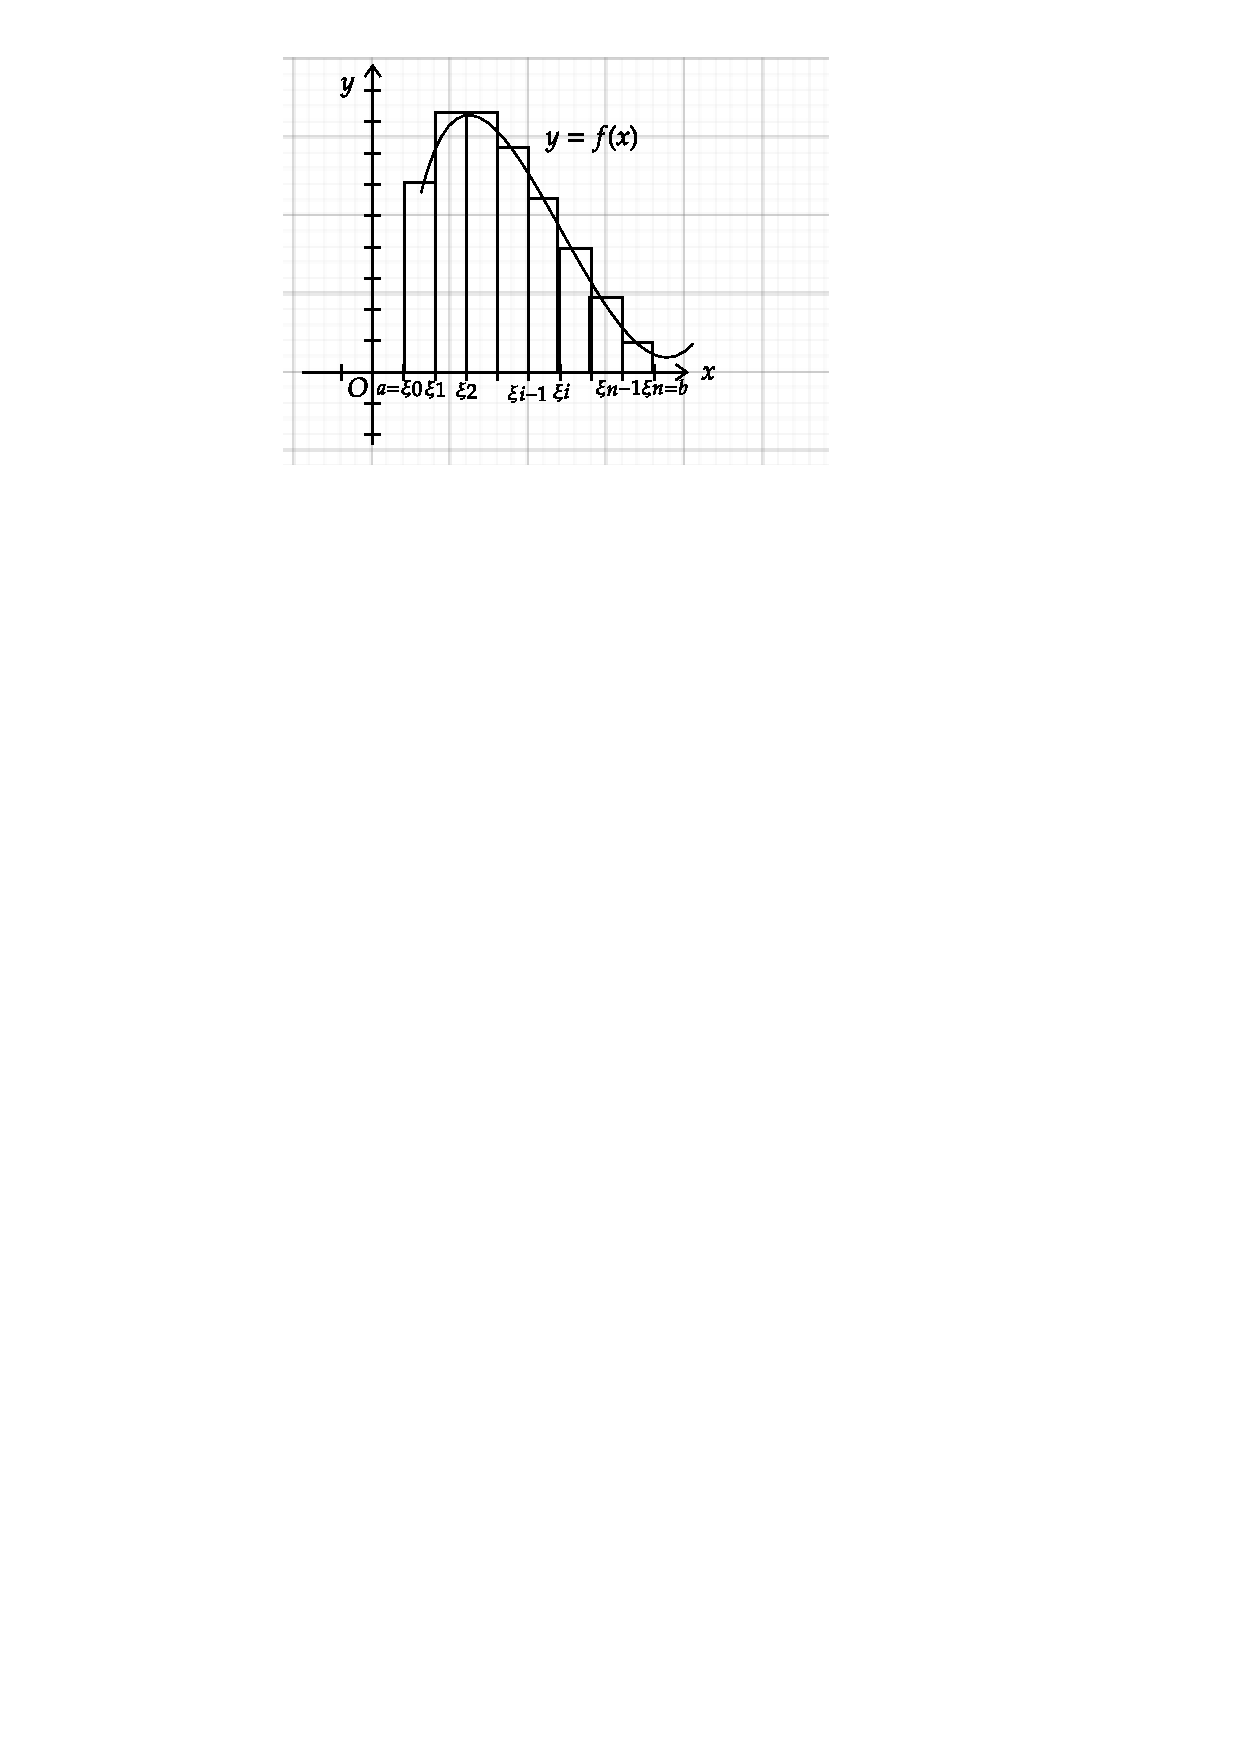
\includegraphics[width=0.4\textwidth]{7.1.1.pdf}
        \end{figure}
        若将式子中的$a,b$ 特殊化为 0,1 这两个数,得出的形式更为简单:
        $$
            \int_0^1f(x)\mathrm{d}x=\lim_{n\to\infty}\sum_{i=1}^nf\biggl(\frac{i}{n}\biggr)\frac{1}{n}\:.
        $$
    \end{defn}
    \begin{them}{定积分的存在定理}{}
        定积分的存在性,也称一元函数的(常义)可积性.这里的“常义”是指“区间有限,函数有界”, 也有人称为黎曼可积性\footnote{此处的可积性与后面的反常积分不同,反常积分是“区间无穷,函数无穷”}.
        \begin{itemize}
            \item 定积分存在的充分条件
                  \begin{enumerate}
                      \item 若$f(x)$在$[a,b]$上连续,则$\int_a^bf(x) dx$存在
                      \item 若$f(x)$在$[a,b]$上单调,则$\int_a^bf(x) dx$存在
                      \item 若$f(x)$在$[a,b]$上\textbf{有界,且只有有限个间断点}\footnote{其实只剩下了可去和跳跃间断点},则$\int_a^bf(x)dx$存在
                            \newline 对于上三个充分条件,可以结合定积分的几何意义来理解,定积分存在就是指的围成的曲边梯形面积能算出来.只要围出来的面积可以算出来,即使$f(x)$在有限个点的函数值发生突变,$f(x)$依然可积.因为在间断点,那条线与$x$轴围成的面积为0,所以第一类间断点不影响总体面积.
                            \begin{center}
                                \tikzset{every picture/.style={line width=0.75pt}} %set default line width to 0.75pt    
                                \begin{tikzpicture}[x=0.75pt,y=0.75pt,yscale=-1,xscale=1]
                                    \draw  (14.71,111.41) -- (207.36,111.41)(49.75,23) -- (49.75,132.3) (200.36,106.41) -- (207.36,111.41) -- (200.36,116.41) (44.75,30) -- (49.75,23) -- (54.75,30) (69.75,106.41) -- (69.75,116.41)(89.75,106.41) -- (89.75,116.41)(109.75,106.41) -- (109.75,116.41)(129.75,106.41) -- (129.75,116.41)(149.75,106.41) -- (149.75,116.41)(169.75,106.41) -- (169.75,116.41)(189.75,106.41) -- (189.75,116.41)(29.75,106.41) -- (29.75,116.41)(44.75,91.41) -- (54.75,91.41)(44.75,71.41) -- (54.75,71.41)(44.75,51.41) -- (54.75,51.41) ;
                                    \draw   ;
                                    \draw [line width=1.5]    (63.36,87) .. controls (92.36,41) and (148.36,91) .. (170.36,34) ;
                                    \draw  [dash pattern={on 4.5pt off 4.5pt}]  (63.36,87) -- (63.36,117) ;
                                    \draw  [dash pattern={on 4.5pt off 4.5pt}]  (170.36,34) -- (170.36,117) ;
                                    \draw  (11.71,257.41) -- (217.36,257.41)(49.12,169) -- (49.12,278.3) (210.36,252.41) -- (217.36,257.41) -- (210.36,262.41) (44.12,176) -- (49.12,169) -- (54.12,176) (69.12,252.41) -- (69.12,262.41)(89.12,252.41) -- (89.12,262.41)(109.12,252.41) -- (109.12,262.41)(129.12,252.41) -- (129.12,262.41)(149.12,252.41) -- (149.12,262.41)(169.12,252.41) -- (169.12,262.41)(189.12,252.41) -- (189.12,262.41)(29.12,252.41) -- (29.12,262.41)(44.12,237.41) -- (54.12,237.41)(44.12,217.41) -- (54.12,217.41)(44.12,197.41) -- (54.12,197.41) ;
                                    \draw   ;
                                    \draw [line width=1.5]    (60.36,233) .. controls (74.18,212.17) and (100.87,234.81) .. (111.36,209) ;
                                    \draw  [dash pattern={on 4.5pt off 4.5pt}]  (60.36,233) -- (60.36,263) ;
                                    \draw  [dash pattern={on 4.5pt off 4.5pt}]  (196.36,172) -- (196.36,255) ;
                                    \draw [line width=1.5]    (112.36,202) .. controls (183.36,201) and (154.36,171) .. (196.36,172) ;
                                    \draw  [dash pattern={on 4.5pt off 4.5pt}]  (112.36,202) -- (112.36,259) ;
                                    \draw   (83.71,222.82) .. controls (83.71,221.44) and (84.69,220.32) .. (85.89,220.32) .. controls (87.1,220.32) and (88.07,221.44) .. (88.07,222.82) .. controls (88.07,224.2) and (87.1,225.32) .. (85.89,225.32) .. controls (84.69,225.32) and (83.71,224.2) .. (83.71,222.82) -- cycle ;
                                    \draw  [fill={rgb, 255:red, 0; green, 0; blue, 0 }  ,fill opacity=1 ] (108.21,169.82) .. controls (108.21,168.44) and (109.19,167.32) .. (110.39,167.32) .. controls (111.6,167.32) and (112.57,168.44) .. (112.57,169.82) .. controls (112.57,171.2) and (111.6,172.32) .. (110.39,172.32) .. controls (109.19,172.32) and (108.21,171.2) .. (108.21,169.82) -- cycle ;
                                    \draw   (150.46,195.82) .. controls (150.46,194.44) and (151.44,193.32) .. (152.64,193.32) .. controls (153.85,193.32) and (154.82,194.44) .. (154.82,195.82) .. controls (154.82,197.2) and (153.85,198.32) .. (152.64,198.32) .. controls (151.44,198.32) and (150.46,197.2) .. (150.46,195.82) -- cycle ;
                                    \draw    (205.33,57.33) -- (296.7,108.36) ;
                                    \draw [shift={(298.44,109.33)}, rotate = 209.18] [color={rgb, 255:red, 0; green, 0; blue, 0 }  ][line width=0.75]    (10.93,-3.29) .. controls (6.95,-1.4) and (3.31,-0.3) .. (0,0) .. controls (3.31,0.3) and (6.95,1.4) .. (10.93,3.29)   ;
                                    \draw    (205.11,185.33) -- (298.56,151.35) ;
                                    \draw [shift={(300.44,150.67)}, rotate = 160.02] [color={rgb, 255:red, 0; green, 0; blue, 0 }  ][line width=0.75]    (10.93,-3.29) .. controls (6.95,-1.4) and (3.31,-0.3) .. (0,0) .. controls (3.31,0.3) and (6.95,1.4) .. (10.93,3.29)   ;
                                    \draw (661,128) node [anchor=north west][inner sep=0.75pt]   [align=left] {$\displaystyle y$};
                                    \draw (212,102) node [anchor=north west][inner sep=0.75pt]   [align=left] {$\displaystyle x$};
                                    \draw (32.4,112.92) node [anchor=north west][inner sep=0.75pt]   [align=left] {$\displaystyle O$};
                                    \draw (-46,78) node [anchor=north west][inner sep=0.75pt]   [align=left] {$ $};
                                    \draw (30.4,17) node [anchor=north west][inner sep=0.75pt]   [align=left] {$\displaystyle y$};
                                    \draw (59,118) node [anchor=north west][inner sep=0.75pt]   [align=left] {$\displaystyle a$};
                                    \draw (165,120) node [anchor=north west][inner sep=0.75pt]   [align=left] {$\displaystyle b$};
                                    \draw (222,249) node [anchor=north west][inner sep=0.75pt]   [align=left] {$\displaystyle x$};
                                    \draw (29.4,258.92) node [anchor=north west][inner sep=0.75pt]   [align=left] {$\displaystyle O$};
                                    \draw (27.4,163) node [anchor=north west][inner sep=0.75pt]   [align=left] {$\displaystyle y$};
                                    \draw (56,264) node [anchor=north west][inner sep=0.75pt]   [align=left] {$\displaystyle a$};
                                    \draw (191,264) node [anchor=north west][inner sep=0.75pt]   [align=left] {$\displaystyle b$};
                                    \draw (311.33,110.67) node [anchor=north west][inner sep=0.75pt]   [align=left] {$\displaystyle \int _{a}^{b} f( x) dx$};
                                \end{tikzpicture}
                            \end{center}
                  \end{enumerate}
            \item 定积分存在的必要条件
                  \begin{enumerate}
                      \item 可积函数必有界,即若定积分$\int_a^bf(x)dx$存在,则$f(x)$在$[a,b]$上必有界. \footnote{当我们任意分割图形底边为若干小段时若$f(x)$在区间$[a、b]$上无界,则至少存在一个小段$\Delta x$,使得“面积”$f(x) \Delta x$无穷大,这样整个曲边梯形的面积就是无穷大,则极限就不存在,所以可积函数必有界}
                  \end{enumerate}
        \end{itemize}
    \end{them}
    \begin{criterion}{定积分的性质}{}
        当$b=a$时,$\int_a^af(x)dx=0$;
        当$a>b$时,$\int_a^bf(x)$d$x=-\int_b^af(x)dx$
        \begin{enumerate}
            \item 求区间长度:假设 $a<b$,则$\int _a^b dx=b-a=L$ ,其中$L$ 为区间$[a,b]$的长度
            \item 积分的线性性质:设$k_{_1}, k_{_2}$为常数,则$\int_{a}^{b}[k_{_1}f(x)\pm k_{_2}g(x)]\mathrm{d}x=k_{_1}\int_{a}^{b}f(x)\mathrm{d}x\pm k_{_2}\int_{a}^{b}g(x)\mathrm{d}x$.
            \item 积分的可加(拆)性:无论$a,b,c$的大小如何,总有$\int_a^bf(x)\mathrm{d}x=\int_a^cf(x)\mathrm{d}x+\int_c^bf(x)\mathrm{d}x$
            \item 积分的保号性:若在区间$[a,b]$上$f(x)\leqslant g(x)$,则有$\int_{a}^{b}f(x)\mathrm{d}x\leqslant\int_{a}^{b}g(x)\mathrm{d}x$.特殊地,有$$\quad\left|\int_a^bf(x)\mathrm{d}x\right|\leqslant\int_a^b\left|f(x)\right|\mathrm{d}x$$
            \item 估值定理:设$M,m$分别是$f(x)$在$[a,b]$上的最大值和最小值,$L$为区间$[a,b]$的长度,则有
                  $$mL\leqslant\int_{a}^{b}f(x)\mathrm{d}x\leqslant ML\:$$
        \end{enumerate}
    \end{criterion}
    \section{定积分的计算}
    \begin{defn}{牛顿莱布尼茨公式}{}
        设函数 $F(x)$是连续函数$f(x)$在$[a,b]$上的一个原函数,则
        $$\int_{a}^{b}f(x)\mathrm{d}x=F(x)\Big|_{a}^{b}=F(b)-F(a)$$
    \end{defn}
    \begin{criterion}{牛顿莱布尼茨公式推广}{}
        \begin{itemize}
            \item 若$f(x)$在$\left[a,b\right]$上有原函数$F(x)$,则$\int_{a}^{b}f(x)\mathrm{d}x=F(b)-F(a)$\footnote{有原函数即可,不需要连续}
            \item 若$f(x)$在$[a,b]$上分段有原函数,如$[a,c)$上有原函数$F_1(x),(c,b]$上有原函数$F_2(x)$,则
                  $$\int_{a}^{b}f(x)\mathrm{d}x=\int_{a}^{c}f(x)\mathrm{d}x+\int_{c}^{b}f(x)\mathrm{d}x=F_{1}(c-0)-F_{1}(a)+F_{2}(b)-F_{2}(c+0)\:.$$\footnote{其实就是以$C$为中心拆成两半进行计算}
                  若$F_1(c-0),F_2(c+0)$存在,则$\int_a^bf(x)dx$收敛。若$F_1(c-0),F_{2}(c+0)$至少有一个不存在,则$\int_a^bf(x)$d$x$发散。
        \end{itemize}
    \end{criterion}
    \section{定积分积分法}
    \subsection{定积分的换元积分法}
    设$f(x)$在$[a,b]$上连续,函数$x=\varphi(t)$满足
    \begin{enumerate}
        \item $\varphi(\alpha)=a,\varphi(\beta)=b$
        \item $x=\varphi(t)$在$[\alpha,\beta]$或$[\beta,\alpha]$上有连续的导数,且其值域为$R_\varphi=[a,b]$,则有$$\int_{a}^{b}f(x)\mathrm{d}x=\int_{\alpha}^{\beta}f[\varphi(t)]\varphi'(t)\mathrm{d}t\:.$$
    \end{enumerate}
    \subsection{定积分的分部积分法}
    $\int_{a}^{b}u(x)v^{\prime}(x)$d$x=u(x)v(x)\Big|_a^{b}-\int_{a}^{b}\nu(x)u^{\prime}(x)$d$x$,这里要求$u^\prime(x),v^{\prime}(x)$在$[a,b]$上连续。
    \begin{conclusion}{定积分分部积分法常用结论}{}
        \begin{itemize}
            \item 区间再现公式:设$f(x)$为连续函数,则$$\int_{a}^{b}f(x)dx=\int_{a}^{b}f(a+b-x)dx$$
            \item $\int_{0}^{\frac{\pi}{2}}\sin^{n}x\mathrm{d}x=\int_{0}^{\frac{\pi}{2}}\cos^{n}x\mathrm{d}x=\begin{cases}\dfrac{n-1}{n} \cdot \dfrac{n-3}{n-2} \cdot \cdots \cdot \dfrac{2}{3} \cdot 1,&n\text{ 为大于 1 的奇数,}\\ \dfrac{n-1}{n} \cdot \dfrac{n-3}{n-2} \cdot \cdots \cdot \dfrac{1}{2} \cdot \dfrac{\pi}{2},&n\text{ 为正偶数 }.\end{cases}$
            \item $\begin{aligned} & \int_0^\pi \sin ^n x \mathrm{~d} x= \begin{cases}2 \cdot \dfrac{n-1}{n} \cdot \dfrac{n-3}{n-2} \cdots \cdot \dfrac{2}{3} \cdot 1, & n \text {为大于} 1 \text {的奇数, } \\ 2 \cdot \dfrac{n-1}{n} \cdot \dfrac{n-3}{n-2} \cdots \cdots \cdot \dfrac{1}{2} \cdot \dfrac{\pi}{2}, & n \text { 为正偶数, }\end{cases} \\ & \int_0^\pi \cos ^n x \mathrm{~d} x= \begin{cases}0, & n \text { 为正奇数, } \\ 2 \cdot \dfrac{n-1}{n} \cdot \dfrac{n-3}{n-2} \cdots \cdots \dfrac{1}{2} \cdot \dfrac{\pi}{2}, & n \text { 为正偶数. }\end{cases} \end{aligned}$
            \item $\int_{0}^{2\pi}\cos^{n}x\mathrm{d}x=\int_{0}^{2\pi}\sin^{n}x\mathrm{d}x=\begin{cases}0\:,&n\text{ 为正奇数,}\\4\cdot\dfrac{n-1}{n}\cdot\dfrac{n-3}{n-2}\cdot\cdots\cdot\dfrac{1}{2}\cdot\dfrac{\pi}{2}\:,&n\text{ 为正偶数 }.\end{cases}$
        \end{itemize}
    \end{conclusion}
    %  ############################ 正文部分
    \ifx\allfiles\undefined
\end{sloppypar}
\end{document}
\fi
